\section{Introduction}
\label{sec:intro}

% Key/value stores remain a fundamental building block of modern
% scale-out service architectures.  Recent trends in primary storage
% technologies, however, are pushing operators to consider ever-more
% disaggregated designs for their in-memory storage systems.
% Concretely, increases in CPU core counts coupled with stagnating DRAM
% density has led to an increased interest in remote memory tiers, where
% some portion of memory is connected to the server over a network.
% Moreover, once disaggregated, memory can be pooled to achieve greater
% cost and power efficiencies.  The challenge facing fully disaggregated
% memory pools, however, is managing concurrent updates in the face of
% client failures and high access latencies.

% While cache-coherent technologies like CXL are beginning to
% become available, RDMA remains the commodity option for
% large-scale in-memory key/value stores.
% Many prior RDMA-based systems opt for a partially
% disaggregated model, in which a CPU core is collocated with
% remote memory to provide the needed
% serialization~\cite{erpc,herd,pilaf,cell,clover,sherman}.
% Fully disaggregated systems rely upon one-sided RDMA atomic
% operations (e.g., compare-and-swap) to resolve data
% races~\cite{rolex,fusee,race} which constrains their design.
% Specifically, RDMA atomic operations can act upon 64 contiguous bits
% of memory at a time at most, leading to implementations that employ
% multi-stage datastructures to support practical key and value sizes.

% In general, existing systems rely upon a high-performance index
% structure to localize key operations and maintain values separately,
% necessitating multiple RDMA operations and network round trips even in
% the absence of contention.  Moreover, given the dominance of
% read-heavy workloads~\cite{rocks-db-workload,facebook-memcached}, most
% systems eschew locks in favor of optimistic update approaches that can
% lead to poor performance under contention.
% In this work we design an index datastructure tailored for the
% constraints of current RDMA hardware.  Specifically, we
% facilitate lock-based updates by decreasing the number of round
% trips required to acquire locks and perform mutating operations.

Resource disaggregation promises improvements in scalability and resource utilization. Main memory
has become a scarce resource in recent years as increased CPU core counts have quickly outpaced
improvements in memory capacity leading to a lower CPU core to memory ratio than at any point in the
last 30 years. Architectures for disaggregated memory have shown that pooling memory leads to much
higher utilization by reducing stranding [huge number of citations]. Critically though many of these
designs forgo sharing memory due to the high cost of synchronization over the network [citation
block]. To realize the full benefit of disaggregated memory designers need a low cost mechanism for
reading and writing to shared resources consistently.

Key/value stores are the current fundamental building blocks for sharing disaggregated memory. In
most cases these systems are built on top of one-sided RDMA and use RDMA atomic operations as a
means to synchronize read and write accesses to remote memory. The main challenge in designing these
systems is efficient serialization. Disaggregation assumes that machines housing pooled DRAM do not
have powerful CPUs. This means that clients must implement their own serialization protocols. When
conflicts occur the cost of reconciliation is high. Most systems use RDMA compare-and-swap to
optimistically commit writes. This approach has two fundamental drawbacks. Firstly atomic writes are
limited to 64 bits - this means that writes for values larger than 64 bits must be done indirectly.
One writes to an uncontended region, and a second to a shared index. Second, the cost of
synchronization is high. In a contended region a CAS may fail as it became state from its last read.

KV store design around indirect reads and writes leads to two fundamental drawbacks 1) All access
requires at least two round trips. Read requires a round trip to read the index and another for the
data. Update, delete and insert operations require at least two if not more. 2) Indirect indexes do
not support complex updates limiting their generality. High performance indexes for RDMA like Cuckoo
and Hopscotch hashes can not be supported as they require locks to update multiple locations in the
index atomically.  Alternatively a lock based index can support inlined operations and complex
updates but can struggle from large critical sections and failure while clients hold locks.


We introduce RCuckoo, a fully disaggregated key/value store based on
cuckoo hashing~\cite{cuckoo} that
uses only one-sided RDMA operations.
RCuckoo builds
around a \emph{dependent hashing} algorithm that makes spatial
locality a tunable parameter.
RCuckoo employs a set of
complimentary techniques that leverage this enhanced locality to deliver higher performance than any prior
disaggregated key/value store while gracefully handling client
failures:

\begin{itemize}
\item{\textbf{Deterministic lock-free reads.}  Cuckoo hashing ensures
  an entry is always located in one of two locations which can be
  read in parallel.}

\item{\textbf{Space-efficient locks} frequently allow clients to acquire necessary 
  locks in a single RDMA operation.}

\item{\textbf{Client-side caching} enables accurate cuckoo-path
  speculation to improve insert performance.}

\item{\textbf{Leased lock acquisitions} allow clients to detect
  and recover from client failures using timeouts.}
\end{itemize}

%% message round-trips for both reads and writes,
%% improving performance for small-object reads and significantly
%% improving writes.


\begin{figure*}[t]
    \centering
    \newcommand{\subfigwidth}{0.32\linewidth}
    % \begin{subfigure}{\subfigwidth}
    %     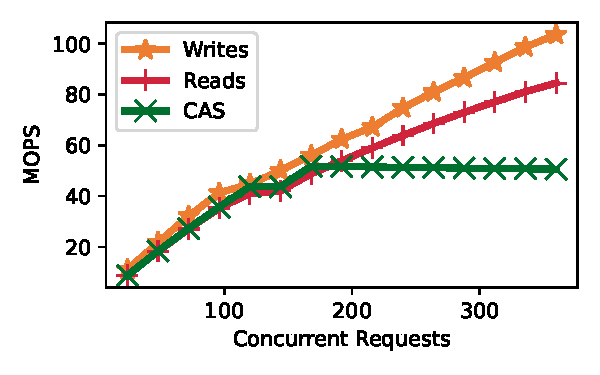
\includegraphics[width=0.99\linewidth]{fig/rdma_concur.pdf}
    %     % \label{fig:optimistic_failures}
    %     % \caption{}
    % \end{subfigure}
    \begin{subfigure}{\subfigwidth}
        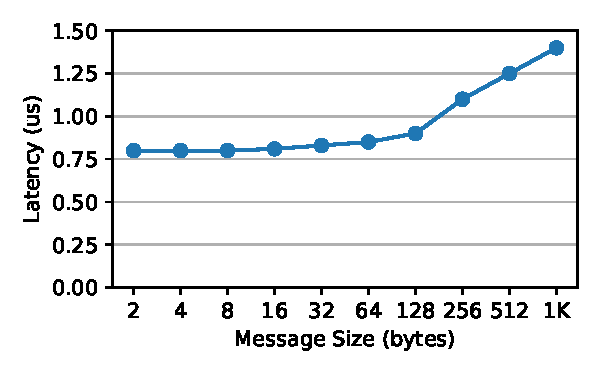
\includegraphics[width=0.99\linewidth]{fig/rdma_latency.pdf}
    \end{subfigure}
    \begin{subfigure}{\subfigwidth}
      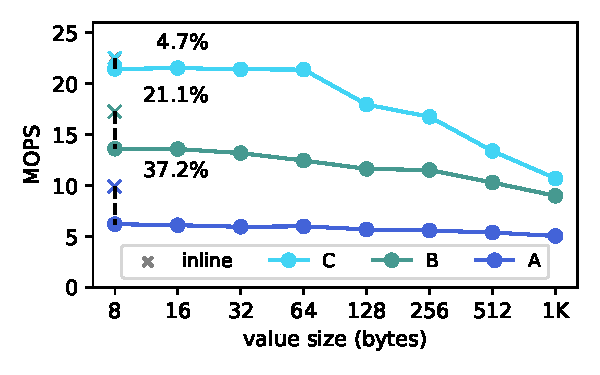
\includegraphics[width=0.99\linewidth]{fig/extent.pdf}
    \end{subfigure}
    \begin{subfigure}{\subfigwidth}
        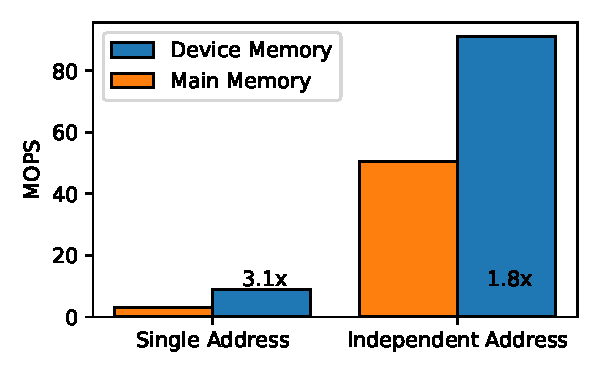
\includegraphics[width=0.99\linewidth]{fig/rdma_cas_throughput.pdf}
    \end{subfigure}
    \vspace{-1em}
    \caption{Basic RDMA performance on our testbed.
    % \textbf{(a)} (64-bit) operations per second;
    \textbf{(a)} operation latency as a function of message size~\cite{rdma-latency}; and
    \textbf{(b)} Extent vs Inline performance on YCSB workloads for small values (C=100\% reads, B=95\%read 5\%write A=50\%read 50\% write).
    \textbf{(c)} compare-and-swap performance on device and main memory.
    }
    \label{fig:rdma-benchmarks}
\vskip -1em
\end{figure*}

Combined with a datastructure design that facilitates aggressive
batching of RDMA operations, these techniques enable RCuckoo to limit
the number of round trips required for all table operations.  In the
common case, reads execute in one or two (for large values) round
trips, uncontested updates and deletes require two round trips, and
the median insert operation involves only two round trips---although
the expected number increases as the table fills.  On our testbed,
RCuckoo delivers comparable or higher performance on small values across the standard set  of YCSB benchmarks than all of the existing disaggregated
key/value stores we consider.  Concretely, with 320 clients RCuckoo
delivers up to a 2.5$\times$ throughput improvement on read-intensive
(YCSB-B) workloads and up to 7.1$\times$ their throughput on
write-intensive (YCSB-A) workloads.  Moreover, RCuckoo's
performance remains high despite 100s of
clients failing per second.
